
In this section, we will provide explanations of the methods, techniques, and procedures employed in our experiments. We will begin by discussing the data preprocessing steps, followed by an explanation of the training process. Finally, we will describe how we evaluated the performance of our models.

\subsection{Engineering For Machine Learning}
In order to streamline our experimental process and minimize effort,
we focused on developing the training and preprocessing code in a way that allows for easy experimentation.
We also utilized tools that enhance efficiency and reproducibility in the research process, reducing time-consuming tasks.
\medskip

We adopted the \texttt{zenml} \cite{zenml} framework to structure our training and preprocessing pipelines.
This framework brings several advantages to our workflow.
One notable benefit is the promotion of modularity in the design of our pipelines.
Each pipeline consists of individual steps, which enhances the code's modularity.
By defining a series of functions with clear inputs and outputs,
we ensure that each step can be easily understood and modified as needed.
Moreover, the \texttt{zenml} web application offers a convenient way to monitor the status of our pipelines.
This feature provides transparency and improves comprehension by providing insights into the outputs generated at each step.
\medskip

For experiment tracking we used the \texttt{MLFlow} framework \cite{mlflow}.
This makes it easy to track all metrics over all experiments.
With \texttt{MLFlow} it is also possible to compare different parameters that were used during training to experimentally find the best combinations.
In \texttt{MLFlow} we save each finished model as an artifact which can be directly served as a server endpoint to start providing end users access to our models.
\medskip

We used the pytorch lightning library. Using patterns such as the \texttt{DataModule} and {LightningModule} to accelerate the
research process. This library abstracts the process of backpropagation and updating parameters.
Furthermore pytorch ligthning \cite{lightning} handles
switching from training devices automatically for example \texttt{cpu} and \texttt{cuda} devices
which decouples the training code from specific hardware.

We made use of the \texttt{typed-settings} library \cite{typed} to allow cleanly structuring and validating settings for models.
This ensures that to train a new version of a model in most cases only adjustments to the configuration file needs to be done.
\texttt{typed-settings} supports passing training settings through toml configuration files, environment variables and command line options.

\subsection{Data Preprocessing}
For the preprocessing of data we created a pipeline which distinguishes between satellite images and radar images to process each following their own needs (See figure \ref{fig:preprocessing}).
\medskip

The pipeline begins by obtaining all necessary files, from a remote storage bucket.
This is done by a Bucket Service class which uses the \texttt{boto3} \cite{boto}
library to interface with the bucket and download files in the required date ranges.
\medskip

In the case of satellite data, the obtained files are compressed in zip files. The pipeline handles the extraction of these files deleting any files which are not needed along the way to ease the storage requirements.
Then we \textit{reproject} the satellite images using the \texttt{satpy} package. This downsampling is done by a combination of cropping and interpolation via the nearest-neighbor algorithm.
\medskip

By reprojecting we reduce the dimensions of each satellite image to \texttt{256 x 256} pixels from it's original dimensions of \texttt{3712 x 3712}.
We also obtain only the geographical area of interest, specified by the coordinates for the lower corner \texttt{(50°0'0"N 0°0'0"E)} and the upper corner \texttt{(55°0'0"N 10°0'0"E)} of the region, this gives us
the area centered on the netherlands with other bordering countries (see figure \ref{fig:reprojection}). Additionally we change the map projection to \textit{Mercator} from the original \textit{Geostationary}.
This is done to have both input and target grids in the same map projections.
After reprojecting we perform a \textit{statistics} step where we aggregate the dataset by finding the minimum and maximum values for each channel see table \ref{tab:channels} for the list of all channels.
The statistics are necessary for the next step which is normalization. During the normalization step we perform the \textit{Min-Max} Normalization (equation 1).

\begin{figure}
  \centering
  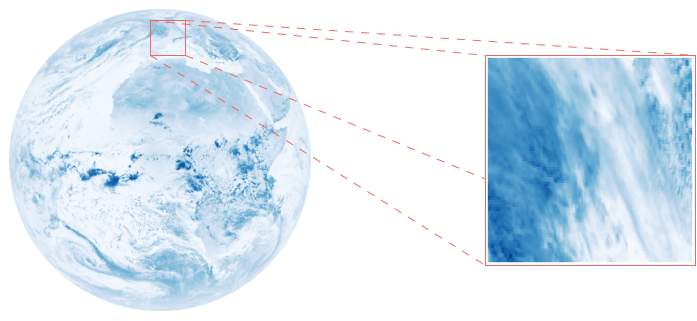
\includegraphics[width=225pt]{./images/reprored.png}
  \caption{Reprojection of Satellite Data: Converting from geostationary projection to mercator projection and reduce to area of interest.}
  \Description{Satellite Image of the earth}
  \label{fig:reprojection}
\end{figure}


\begin{equation}
  x_{normalized} = \frac{x-min(\bar{x})}{max(\bar{x})-min(\bar{x})}
\end{equation}

After finalizing the normalization step we sample an image from the dataset which is visualized to check for errors in the pipeline.
\medskip

The radar pipeline begins with the downloaded \texttt{h5} files
each is converted to decibels relative to Z (dBZ) (equation 8) from a \textit{grayscale} unit ranging from 0 to 255.
Using decibels relative to Z adds to the interpretability  and makes it easier to weight loss functions and metrics
according to the level of precipitation. The drawback of this is that to plot the image or perform image transformations many
existing libraries make the assumption of either \textit{grayscale} or \textit{rgb} images, therefore to make use of these resources we must sometimes convert back to the \textit{grayscale} unit. 

\begin{equation}
  dBZ(x) = x \cdot 0.5 - 32
\end{equation}

The preprocessing pipeline then splits into two, one step will normalize values between 0 and 1 using \textit{Min-Max} normalization and the other step will use levels of \textit{dBZ} to create discrete ranges of precipitation to use as classes during training \ref{tab:classes}.
Finally the current images in the pipeline are resized using the nearest neighbor algorithm, to avoid changing the class values with bilinear interpolation.
Next identically to the satellite pipeline we sample and visualize a radar image for verification purposes.

\begin{figure}
  \centering
  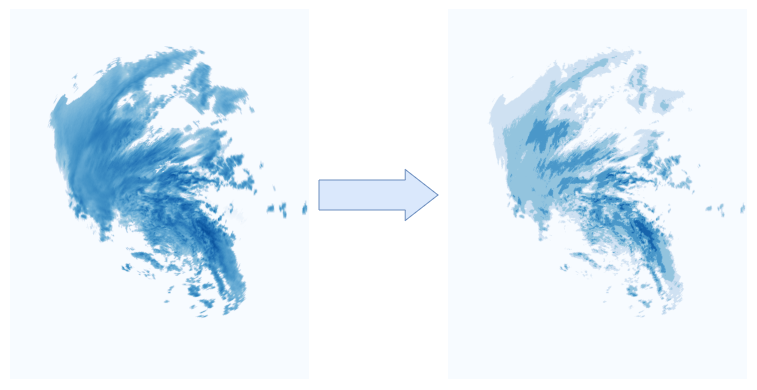
\includegraphics[width=225pt]{./images/bins.png}
  \caption{Preprocessed Radar Reflectivity Data For 2023-03-10 at 11:55 UTC. Left with normalized data and right with pixels put into 8 different rainfall intensity classes.}
  \Description{Satellite Image of the earth}
  \label{fig:bins}
\end{figure}


\begin{figure}
  \centering
  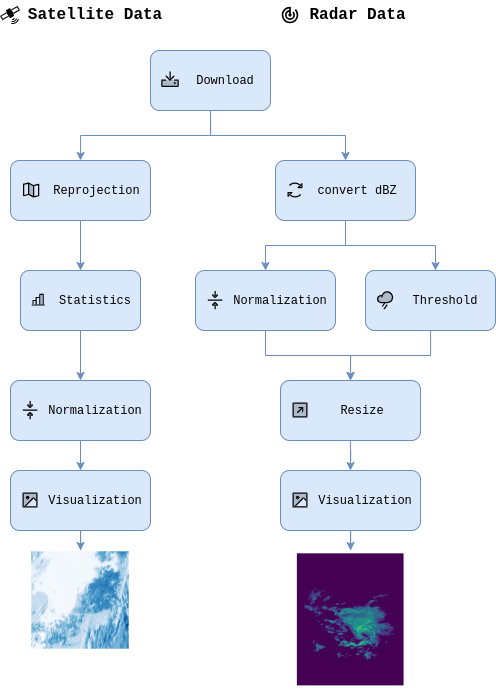
\includegraphics[width=225pt]{./images/prepro.png}
  \caption{Data Preprocessing Pipeline: Satellite Data and Radar data preprocessed separately}
  \Description{Satellite Image of the earth}
  \label{fig:preprocessing}
\end{figure}

\subsection{Proposed Model Architectures}

The 3D U-Net based model is given a input patch of dimension $8\times11\times256\times256$. The U-Net model produces a segmented image for each slice of the depth dimension.
Therefore we added an additional 3D convolution after the normal U-Net architecture which reduces the output of the network from the shape $8\times8\times256\times256$ to the desired $1\times8\times256\times256$ or in the case of regression to $1\times256\times256$
\medskip


For ConvLSTM models, we start with 3 layers of Convolutional LSTMs
with 64 filters that use a kernel size of 3.
Then the short term memory of the last layer is passed to three 2D Convolutional Layers.
The first Convolutional layer reduces the amount of channels to 32, the second to 16 and the last one to either 8 or 1 for classification and regression respectively.
In the intermediate layers a ReLU \cite{relu} activation function is performed.

\subsection{Experimental Setup}
We trained each model for 50 epochs. The batch size was set to 1 because of memory constraints. We used the \textsc{Adam} algorithm for optimization from Kingma et al \cite{kingma-2014}.
All model were trained on a single NVIDIA GeForce RTX 2070 SUPER GPU. We used different losses for classification and regression.
First we used Multi-Class CrossEntropyLoss for classification this first applies a log softmax activation function which normalizes the
outputs produced by our models. Then it calculates the cross entropy loss between the normalized input and the target.
For regression we used the MSE loss. To address class imbalance in the data we added weights for the CrossEntropyLoss. These weights were
obtained by finding the frequencies of the classes in the dataset as follows:

\begin{equation}
  weight(c) = 1 - \frac{1}{h\times w \times n} \times \sum_{i=1}^n \sum_{j=1}^h \sum_{k=1}^w [Y_{ijk} = c]
\end{equation}

We decided to conduct our experiments using $t = 5$, allowing for 1 hour and 15 minutes of temporal data, $h = 256$, $w = 256$, and $c = 12$.

We created 2 different types of datasets for use in the experiments.
The first type is a sequence dataset, this dataset does not repeat any satellite files. It increments the starting point at each sample
by the length of the satellite sequence. On the other hand to make use of all the available data we created a sliding sequence dataset which increments the starting point of the sequences by 1 meaning that the sequence moves by
1 satellite image forward. We have also handled aligning the satellite and corresponding radar target based on their timestamps. 

\subsection{Performance Evaluation}

To evaluate the performance of our models we implemented several metrics. Each of these metrics can be used to measure
the quality of a trained model. Utilizing a range of metrics allows us to better analyze the performance of a particular machine learning model.
Metrics that are used to measure the performance of classification problems are different from the metrics that are used for regression. Note that we
give the formulas that are used to calculate the metric for each image, in the reported results these metrics have been averaged over the entire test dataset.

\subsubsection{Regression Evaluation Metrics}
Regression metrics are often error functions, these functions calculate the distance between prediction and target values. 
When predicting more than one value, we can extend the definition of an error function
by calculating the mean or sum of all distances, the distances themselves are calculated with a certain distance metric for 2 values that are in the same position in the prediction and target.
This is an important distinction when considering that we predict a $h \times w$ image, to calculate the distance between the prediction and target, we will calculate the distance between each pixel then divide it by the number of pixels in the image.

The simplest metric is the \textit{Mean Absolute Error} (equation 3). It takes the absolute value
of the distance between to values since the sign of the error does not affect it's importance.
The mean average error is not differentiable at $x = 0$.

\begin{equation}
  MAE = \frac{1}{h \times w}\sum_{i=0}^h\sum_{j=0}^w |\hat{y_{ij}} -y_{ij}|
\end{equation}

A common regression metric is \textit{Mean Squared Error} (equation 4). MSE squares the distance between two values, so it is always positive and
becomes larger exponentially faster than MAE as the distance between the two values increases.

\begin{equation}
  MSE = \frac{1}{h\times w}\sum_{i=0}^h\sum_{j=0}^w (\hat{y_{ij}} -y_{ij})^2
\end{equation}

MSE punishes outliers more severely and is harder to interpret than MAE because the unit of the error is the squared original unit for example in our case (dBZ) becomes ($dBZ^2$).
The root mean squared error solves the problem of MSE producing uninterpretable units by taking the root of the MSE (equation 5).
\begin{equation}
RMSE = \sqrt{MSE}
\end{equation}

Some metrics have been designed for the task of precipitation nowcasting itself, what is particular about this case is that we place more
importance on predicting the outliers than the overall data. This is because extreme values of rain are the most important to predict correctly as these cause the
most damage to society. Shi et al. \cite{shi2017deep} created \textit{BMAE} (equation 6) and \textit{BMSE} (equation 7) because of this.
These metrics weight errors higher as the target pixel value increases. 

\begin{equation}
BMAE = \frac{1}{h\times w}\sum_{i=0}^h\sum_{j=0}^w weight(y_{ij}) \cdot |\hat{y_{ij}} - y_{ij}|
\end{equation}

\begin{equation}
BMSE = \frac{1}{h\times w}\sum_{i=0}^h\sum_{j=0}^w weight(y_{ij}) \cdot (\hat{y_{ij}} -y_{ij})^2
\end{equation}


\subsubsection{Classification Evaluation metrics} Many classification metrics are based on the \textit{Confusion Matrix}.
The simplest case is a binary classification here a model predicts between two classes suppose we call them 
\textit{positive} and \textit{negative}. There are two possibilities for this output
it can be either \textit{true} or \textit{false}. Thus there exist 4 disjoint sets ($TP$, $TN$, $FP$ and $FN$) all subsets of $\hat{Y}$ the set of all predictions.
Calculating values based on the cardinality of these sets helps us understand the performance of a classification model.
Accuracy is a intuitive metric, it is defined as the fraction of correct classifications over the total amount of classifications.  

\begin{equation}
  Accuracy = \frac{|TP| + |TN|}{|TP| + |FP| + |TN| + |FN|}
\end{equation}


The precision brings the focus on predicting a false positive.
Precision can be a useful measure when we try to measure if a model
is giving too many incorrect positive predictions.

\begin{equation}
  Precision = \frac{|TP|}{|TP| + |FP|}
\end{equation}

The recall gives the score focusing on when the model predicts a false negative.
Recall can be useful when we want to know if the model is predicting too many incorrect negative predictions.
\begin{equation}
  Recall = \frac{|TP|}{|TP| + |FN|}
\end{equation}

The F1 score captures the trade-off between precision and recall, offering a single metric to measure the model's effectiveness.

\begin{equation}
  F1Score = 2 \times \frac{Precision \times Recall}{Precision + Recall}
\end{equation}

The Jaccard index, also known as intersection over union (IoU) created by Jaccard \cite{paul},
Can be used to evaluate a model's performance particularly for image segmentation,
it quantifies the overlap between the predicted positive instances and the actual positive instances.
The Jaccard index is particularly useful when evaluating models on imbalanced datasets, where it can provide a robust measure of performance by focusing on the correct prediction of positive instances while discounting true negatives.

\begin{equation}
  Jaccard Index = \frac{|TP|}{|TP| + |FP| + |FN|}
\end{equation}
\medskip

These metrics can be extended from the binary classification case that has two classes to a general definition for n classes by redefining $TP$, $FP$, $FN$ and $TN$.

Another important remark is that for images, since each pixel is classified, the metrics are first calculated at the image level, then averaged over the number of samples.